\chapter{Régression polynomiale}

L'objectif de cet exercice est d'appréhender la méthode des moindres carrés linéaires pour estimer les paramètres d'un modèle polynomial à partir de données expérimentales.

\section{Construction du jeu de données}

Pour évaluer les performances des méthodes numériques, il est d'usage de simuler des jeux de données via un modèle dont on connait la \guillemotleft vraie\guillemotright\footnote{La notion de valeur \guillemotleft vraie\guillemotright des paramètres n'a aucun sens en pratique car cela supposerait qu'il y a un \guillemotleft vrai\guillemotright modèle; or un modèle mathématique, aussi fin soit-il, n'est qu'une approximation de la réalité qui est trop complexe pour être parfaitement modélisée.} valeur. Cette \guillemotleft vraie\guillemotright\, valeur du vecteur des paramètres n'est bien sûr pas utilisée dans la procédure de résolution du problème posé.

\begin{enumerate}
	\item Pour \texttt{x=(0:0.5:15)';} de dimension $N\times 1$, simuler le modèle polynomial
	\eq{
		\bm{y} = h_0 + h_1\bm{x} + h_2\bm{x}^2 + h_3\bm{x}^3 + h_4\bm{x}^4
	}
	pour un vecteur des paramètres vais, de dimension $p\times 1$, donné par
	\eq{
		\texttt{h = [500; 10; -10; -5; 0.4];}
	}
	Représenter $\bm{y}(\bm{x})$ à l'aide de la commande \texttt{plot}.
	
\item[\textcolor{blue}{Solution.}] \textcolor{blue}{Pensez à toujours commenter votre code, et à donner des noms aux paramètres dans vos scripts, de manière à ce que votre code soit lisible et flexible. Evitez les accents dans vos commentaires.}
\begin{lstlisting}
% TP1: Regression polynomiale

%% 1.1 Construction du jeu de données
x = (0:0.5:15)'; 		% grille de discrétisation (vecteur colonne)
N = length(x); 			% taille de la grille

h = [500; 10; -10; -5; 0.4];	% coefficients du polynome

y = h(1)*x.^0 + h(2)*x + ...    % vecteur des mesures
    h(3)*x.^2 + h(4)*x.^3 + ...
    h(5)*x.^4;

% affichage
clf, plot(x,y,'-.','linewidth',2,'markersize',10);
legend('Echantillons non bruités (inconnus)');
\end{lstlisting}

\begin{figure}[h]
\centering
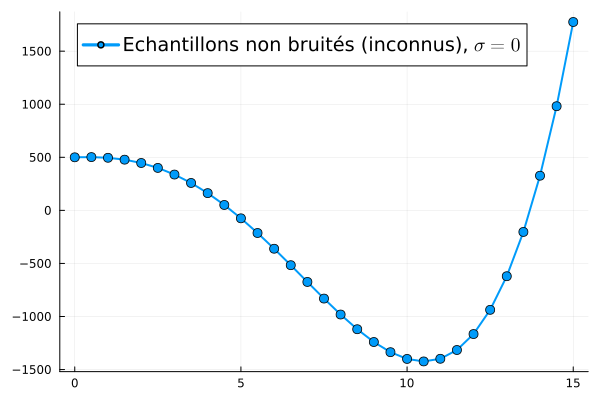
\includegraphics[width=0.5\textwidth]{code/mesures_sans_bruit}
\caption{Données non bruitées (gauche) et bruit seul (droite)}
\end{figure}

\item Pour s'approcher de la réalité, les incertitudes (souvent qualifiées de bruit) sur les mesures sont simulées par une suite stationnaire\footnote{L'hypothèse de stationnarité traduit le fait que l'on suppose que moyenne et variance des incertitudes ne varient pas au cours du temps. Il s'agit ici d'une suite de variables aléatoires indépendantes et indetiquement distribuées, cette terminologie est souvent abrégée par i.i.d.. Lorsque la moyenne est nulle, l'indépendance des variabels aléatoires confère à la densité spectrale du bruit une propriété particulière et l'on parle alors de bruit blanc.} de N variables aléatoires distribuées selon une lo normale $\Nn(\mu,\sig^2)$ de moyenne $\mu=0$ et de variance $\sig^2 = 10^2$: \texttt{b = mu + sigma*randn(N,1);}. Ces incertitdes $\bm{b}$ sont supposées additives et les observaitons disponibles sont notées
	\eq{
		\bm{y}_b = \bm{y} + \bm{b}.
	}
	
Représenter les signaux $\bm{y}_b$ et $\bm{b}$ et relancer plusieurs fois le code. Que constatez-vous?

\item[\textcolor{blue}{Solution.}]
\begin{lstlisting}
mu  = 0; 	% moyenne du bruit
sigma = 10;	% ecart-type du bruit
b = mu + sigma*randn(N,1); 	% bruit gaussien centre

yb = y + b;	% signal bruite

% affichage
clf;
subplot(1,2,1), plot(x,y,'-.','linewidth',2,'markersize',10);
hold on, plot(x,yb,'-x','linewidth',2,'markersize',10);
%
subplot(1,2,2), plot(x,b,'linewidth',2);
\end{lstlisting}

\begin{figure}[h]
\centering
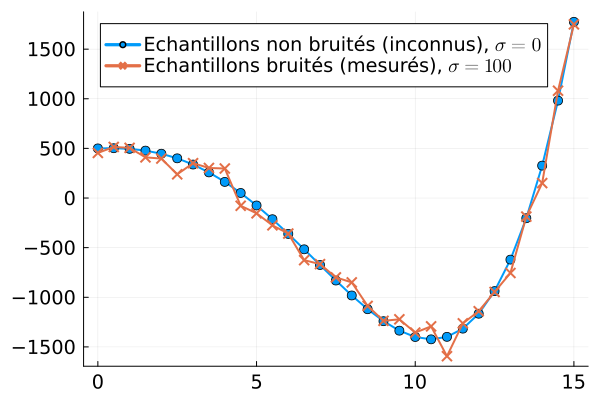
\includegraphics[width=0.4\textwidth]{code/mesures_bruit}
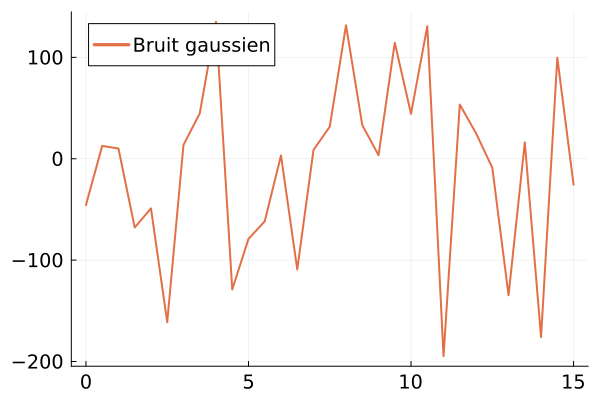
\includegraphics[width=0.4\textwidth]{code/bruit_seul}
\caption{Données bruitées}
\end{figure}

\textcolor{blue}{Afin de relancer plusieurs fois ce code facilement, on peut l'insérer dans une boucle \texttt{for}. Afin de simplement visualiser le résultat à chaque itération, on peut par exemple indiquer à Matlab \texttt{drawnow} (pour qu'il dessine bien chaque fois), et \texttt{pause(0.2)}, pour qu'il fasse une pause de 0.2 secondes à chaque itération.}
\begin{lstlisting}
mu  = 0; 	% moyenne du bruit
sigma = 100;	% ecart-type du bruit

n_tries = 10;
for i=1:n_tries
	b = mu + sigma*randn(N,1); 	% bruit gaussien centre
	yb = y + b; 	% signal bruite
	
	% affichage
	clf;
	subplot(1,2,1), plot(x,y,'-.','linewidth',2,'markersize',10);
	hold on, plot(x,yb,'-x','linewidth',2,'markersize',10);
	%
	subplot(1,2,2), plot(x,b,'linewidth',2);
	
	drawnow;
	pause(0.2);
end
\end{lstlisting}

\textcolor{blue}{On constate que les observations bruitées sont bien sûr différentes à chaque fois: on modélise bien un aléa sur nos mesures. Afin d'observer visuellement l'effet du bruit sur les graphiques, j'ai choisi $\sigma=100$ dans les tests.}

\item Calculer l'énergie du bruit $W_b$ puis modifier la variance de celui-ci. Que constatez-vous?

\item[\textcolor{blue}{Solution.}] \textcolor{blue}{Traçons la valeur de $W_b$ en fonction de l'écart-type $\sigma$ du bruit, pour une série de valeurs de $\sigma$ (en échelles logarithmiques).}
\begin{lstlisting}
n_scales = 4;
Wb = zeros(n_scales,1);  % vecteur dans lequel on stockera les valeurs
for scale = 0:(n_scales-1)
	sigma = 10^scale; % ne pas donner le meme nom qu'avant
	b_test = mu + sigma*randn(N,1); % idem
	
	Wb(scale) = 1/N * norm(b_test)^2; % energie du bruit (stockee)
end

loglog(10.^(0:(n_scales-1)), Wb, 'linewidth', 2); % echelle log en x et en y
\end{lstlisting}
\end{enumerate}

\begin{figure}[h]
\centering
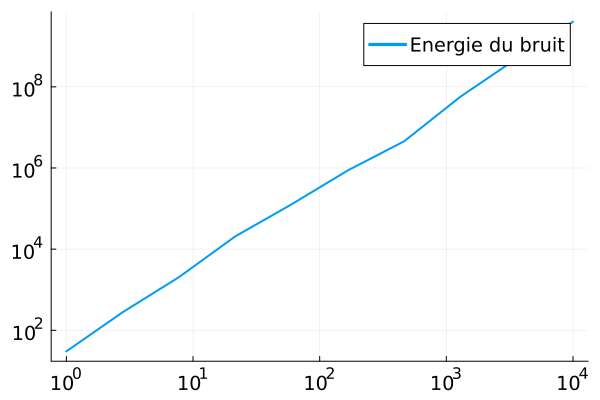
\includegraphics[width=0.4\textwidth]{code/Wb}
\caption{Energie du bruit en fonction de $\sigma$}
\end{figure}

\textcolor{blue}{On constate que l'énergie du bruit croît linéairement avec $\sigma$.}

\section{Moindres carrées linéaires}
\begin{enumerate}
\item Construire la matrice de Vandermonde $\bm{X}$ à partir du vecteur $\bm{x}$.
	
\item[\textcolor{blue}{Solution.}] \textcolor{blue}{La matrice de Vandermonde $\bm{X}$ est simplement la matrice du système liant $\bm{y}$ et $\bm{h}$:
\eq{
	\bm{X} = \begin{bmatrix} 
		1 & x_1 & x_1^2 & \ldots & x_1^4\\
		1 & x_2 & x_2^2 & \ldots & x_2^4\\
		\vdots & \vdots & \vdots & & \vdots\\
		1 & x_N & x_N^2 & \ldots & x_N^4\\
		\end{bmatrix}
}
En Matlab, cela donne:}
\begin{lstlisting}
%%1.2 Moindres carres lineaires
X = [x(:).^0, x(:), x(:).^2, x(:).^3, x(:).^4]; % matrice de Vandermonde
\end{lstlisting}
\textcolor{blue}{La commande \texttt{(:)} permet de s'assurer que le vecteur est sous forme colonne. On vérifiera facilement que $\bm{y} = \bm{X}\bm{h}$.}
	
	\item Déterminer le vecteur $\hat{\bm{h}}$ en utilisant la formulation matricielle des moindres carrés et comparer le résultat obtenu avec la valeur \guillemotleft vraie\guillemotright\, des paramètres. L'instruction \texttt{inv} permet d'inverser une matrice.
	\item[\textcolor{blue}{Solution.}] \textcolor{blue}{La solution des moindres carrés s'obtient via la pseudo-inverse de la matrice $\bm{X}$ du système. Lorsque la matrice est de rang colonne plein (c'est-à-dire lorsque le rang de la matrice est égal à son nombre de colonnes, ce qui est très souvent le cas pour des matrices avec peu de colonnes et beaucoup de lignes), la pseudo-inverse est donnée par la formule
	\eq{
		\bm{X}^\dagger = (\bm{X}^\top\bm{X})^{-1}\bm{X}^\top.
	}
	Il ne reste plus qu'à appliqer cette formule en Matlab.}
\begin{lstlisting}
% pseudo-inverse avec la fonction inv
X_pinv = inv(X'*X)*X';

% estimateur des moindres carres
h_est1 = X_pinv * y;	
\end{lstlisting}
	
	\item Dans le cas général, il n'est pas recommandé d'utiliser la programmation via inv qui est coûteuse en termes de calcul et peut souffrir de problèmes de conditionnement. Plusieurs alternatives sont alors possibles :
	
\begin{lstlisting}
% *******************************
% moindres carres via élimination gaussienne
h_est2 = (X'*X)\X'*y_b;

% *******************************
% moindres carres via factorisation QR
[Q,R] = qr(X);
QTY = Q'*y_b;
opts_UT.UT = true;
h_est3 = linsolve(R,QTY,opts_UT);
Cond_QR = cond(R);

% *******************************
% moindres carres via SVD
[U,S,V] = svd(X,'econ');
h_est4 = V*inv(S)*U'*y_b;
Cond_SVD = cond(S);

% *******************************
% moindres carres via pseudo-inverse (obtenue apres SVD)
h_est5 = pinv(X)*y_b;
\end{lstlisting}

Tester ces différentes alternatives. En principe, les résultats devraient être identiques.

\medbreak
Dans le cas général il convient d'utiliser les approches fondées sur une factorisation QR ou sur une décomposition en valeurs singulières SVD. Si la SVD est plus complexe que la décomposition QR elle fournit le conditionnement du problème et permet la régularisation de problèmes mal conditionnés.

\item Afficher la matrice $\bm{S}$ des valeurs singulières et vérifier que le rapport des valeurs singulières extrêmes donne le conditionnement au sens de la norme 2.
\item[\textcolor{blue}{Solution.}] \textcolor{blue}{La matrice étant diagonale, on affiche ses valeurs diagonales non nulles.}
\begin{lstlisting}
% Affichage des valeurs singulières
s_vals = diag(S);
semilogy(s_vals(s_vals>0), '-.', 'linewidth', 2, 'markersize', 10);
\end{lstlisting}
\begin{figure}[h]
\centering
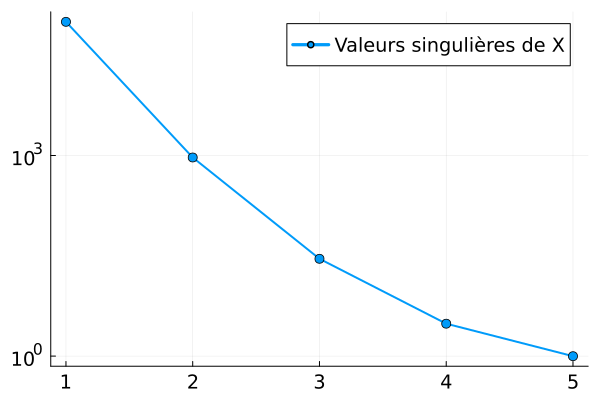
\includegraphics[width=0.4\textwidth]{code/sing_values}
\caption{Valeurs singulières (non nulles)}
\end{figure}
\textcolor{blue}{On constate que la matrice est mal conditionnée: le rapport $\sigma_{\max}/\sigma_{\min}$ est de l'ordre de $10^5$. On vérifie facilement que ce ratio est égal au conditionnement de la matrice pour la norme 2 (fonction \texttt{cond} de Matlab).}
\begin{lstlisting}
cond1 = max(s_vals)/min(s_vals(s>0));
cond2 = cond(X);

fprintf('Le rapport des valeurs singulieres extremes est: %.6d\n Le conditionnement obtenu via la fonction cond est: %.6d\n\n',cond1,cond2);
\end{lstlisting}
\textcolor{blue}{En pratique, cela signifie que la solution estimées par les moindres carrés (sans régularisation, donc à partir de la seule pseudo-inverse) sera instable en présence de bruit.}

\item Calculer et représenter la sortie estimée $\hat{\bm{y}}(x)$ ainsi que les résidus $\bm{\eps}(x) = \bm{y}_b(x) - \hat{y}(x)$.
\item[\textcolor{blue}{Solution.}] \textcolor{blue}{La sortie estimée se déduit immédiatement à partir des coefficients estimés \texttt{h\_est} (avec la méthode que vous préférez) et de la matrice $X$.}
\begin{lstlisting}
% Sortie estimee
y_est = X*h_est;

# Affichage
clf;
subplot(1,2,1), plot(x,y,'-.','linewidth',2,'markersize',10);
hold on;
plot(x,yb,'-x','linewidth',2,'markersize',10);
plot(x,y_est,'-o','linewidth',2,'makersize',10);
legend('Vrais échantillons','Echantillons bruités','Reconstruction');

subplot(1,2,2), plot(x,yb-y_est,'linewdth',2);
legend('Résidus');
\end{lstlisting}
\begin{figure}[h]
\centering
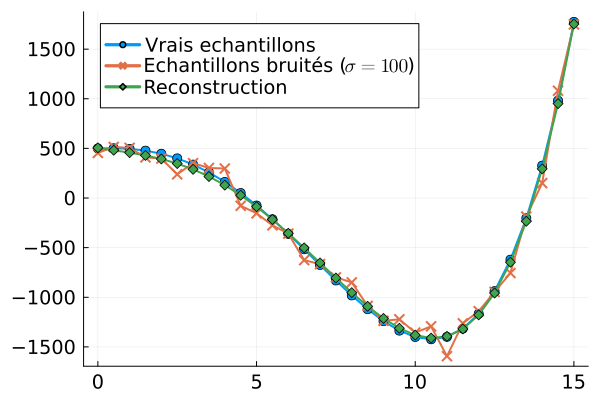
\includegraphics[width=0.4\textwidth]{code/reconstruction}
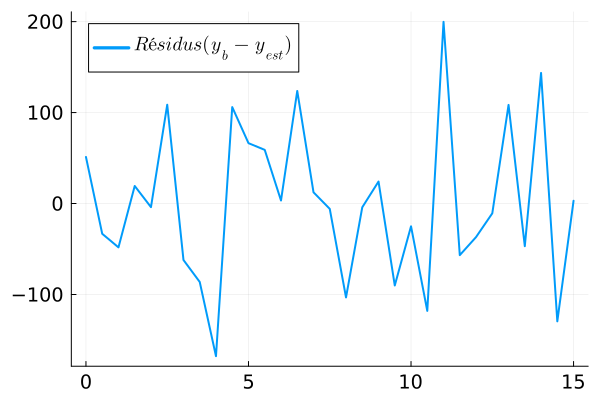
\includegraphics[width=0.4\textwidth]{code/residus}
\caption{Signal reconstruit (gauche) et résidu (droite)}
\end{figure}

\item Que vaut le minimium du critère d'optimisation? Comparer cette valeur à l'énergie du bruit additif calculée précédemment $W_b$.
\item[\textcolor{blue}{Solution.}]

\item Tester également le cas où il n'y a pas de bruit sur les données.
\item[\textcolor{blue}{Solution.}]

\section{Sélection de l'ordre du polynôme}

Lorsque l'on cherche à ajuster un polynôme de degré $d$ à des données expérimentales, l'ordre de ce polynôme est généralement inconnu. Se pose alors le problème de sélection de l'ordre le plus approprié qui peut se formuler comme un problème d'optimisation discrète : rechercher le meilleur ordre au sens d'un certain critère.

\begin{enumerate}
	\item Considérons dans un premier temps que le critère retenu soit celui des moindres carrés. Calculer les valeurs de ce critère pour $d$ variant de $1$ à $10$. Que constatez-vous? A partir de quelle valeur de $d$ ce critère pourra-t-il être nul?
	\item[\textcolor{blue}{Solution.}] \textcolor{blue}{On constaterait que le critère diminue avec $d$. Lorsque $d=N+1$ où $N$ est le nombre de points, on est sûr que l'erreur des moindres carrés sera à zéro, car il existe toujours un polynôme de degré $(N+1)$ qui interpole les $N$ points (le polynôme interpolateur de Lagrange). Vous pourrez facilement vous convaincre de ce résultat en essayant pour des petites valeurs de $N$ (1 ou 2). 
	%
Le critère des moindres carrés seul n'empêche pas le phénomène de \emph{surapprentissage}, qui correspond au cas où le modèle colle trop aux données et n'est plus généralisable: ici par exemple, un modèle qui interpole toutes les données bruitées sera un très mauvais estimateur du polynôme ayant servi à générer les données (de degré 4). 
%
Pour remédier à cela, il faut soit trouver des heuristiques sur le modèle (comme le critère d'Akaike ci-dessous), soit recourir à de la régularisation (cf TP 2).}
	\begin{figure}[h]
	\centering
	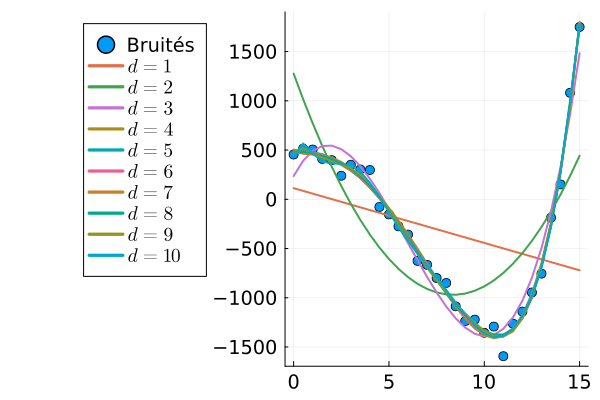
\includegraphics[width=0.4\textwidth]{code/degres.png}
	\caption{Reconstruction pour différents degrés de polynôme}
	\end{figure}
	
	\item Afin de palier l'inconvénient illustré à la question précédente, les techniques de sélection d'ordre s'appuient sur des critères qui pénalisent le nombre de paramètres $p$ afin de
privilégier des modèles parcimonieux (pour cet exercice $p = d + 1$). En effet, l'incertitude d'estimation qui pèse sur chaque paramètre s'accroît avec le nombre de paramètres (l'information disponible via les données, qui est fixe, se répartit sur un plus grand nombre d'entre eux).
	
	Le critère d'information d'Akaike (AIC) permet de réaliser cette sélection d'ordre en retenant celui qui minimise
	\eq{
		AIC = 2\ln(\norm{\bm{\eps}}_2^2) + 2p.
	}
	Déterminer l'ordre du polynôme qui minimise le critère d'information d'Akaike.
	\item[\textcolor{blue}{Solution.}] \textcolor{blue}{On calcule le critère d'Akaike tel que défini dans le sujet, et on trace ses valeurs en fonction du degré $d$ pour $d$ allant de $1$ (approximation linéaire) à 10 (approximation par un polynôme de degré 10).}
\begin{lstlisting}
% Evaluation du critere d'Akaike
dmax = 10;
akaike = zeros(dmax,1);
for d=1:dmax
	Xd = x.^(0:d);	% matrice de Vandermonde d'ordre d
	hd = pinv(Xd)*yb; 	% coefficients estimes par moindres carres
	yd = Xd*hd; 	% signal reconstruit avec le modele d'ordre d
	
	res = yb-yd; 	% residus a l'ordre d
	
	akaike(d) = 2*log(norm(res)^2) + 2*(d+1);
end

plot(1:dmax,akaike,'linewidth',2);
legend('Critère d Akaike');
xlabel('Degré du polynôme (modèle)');
\end{lstlisting}
	\begin{figure}[h]
	\centering
	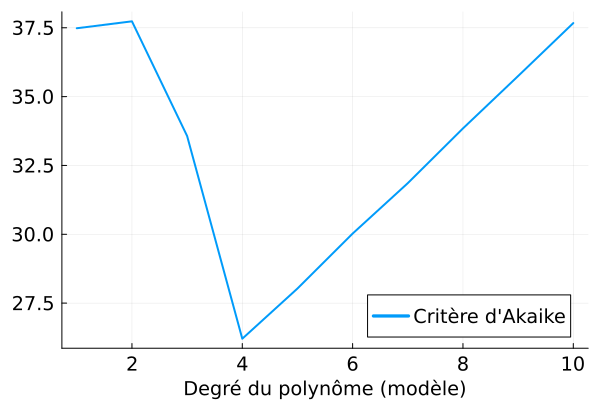
\includegraphics[width=0.4\textwidth]{code/akaike10.png}
	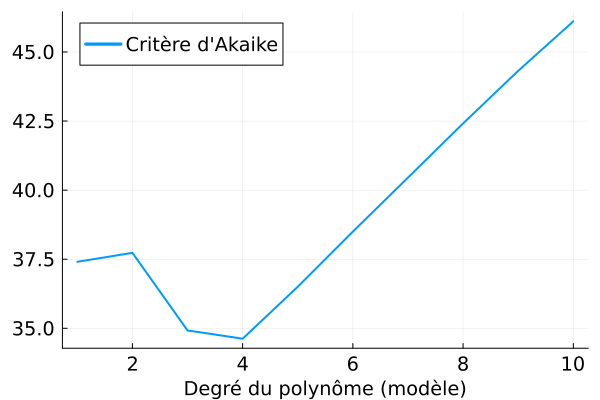
\includegraphics[width=0.4\textwidth]{code/akaike.png}
	\caption{Critère d'Akaike, dans le cas $\sigma=10$ (gauche) et $\sigma=100$ (droite)}
	\end{figure}
\end{enumerate}
\textcolor{blue}{Je vous montre les résultats pour deux intensités de bruit. On voit que lorsque le bruit est trop grand, le critère d'Akaike ne retrouvera pas toujours la bonne valeur du degré (4 dans notre cas), comme on l'observe sur la figure de droite (où le valeur du degré donnant le plus petit critère est 3).}

\end{enumerate}
